\documentclass{article}
\usepackage[utf8]{inputenc}
\usepackage{graphicx}
\usepackage[margin=2.5cm]{geometry}
\usepackage{eso-pic}
\usepackage{hyperref}
\usepackage{wrapfig}
\usepackage{lipsum}
\AddToShipoutPictureBG{%
    \AtPageLowerLeft{
        % \hspace{1cm}
        
\includegraphics[width=4.5cm]{img/Java-Hutts2.png}
    }
}
\title{Tender: Company - Project Name}
\date{May 2017}
\begin{document}

\makeatletter
    \begin{titlepage}
        \begin{center}
            
\includegraphics[width=0.7\linewidth]{img/up.png}\\[4ex]
            {\huge \bfseries \@title }\\[2ex]
            {\LARGE \textbf{Team:} Java the Hutts}\\[2ex]
            {\LARGE \@date}\\[2ex]
            {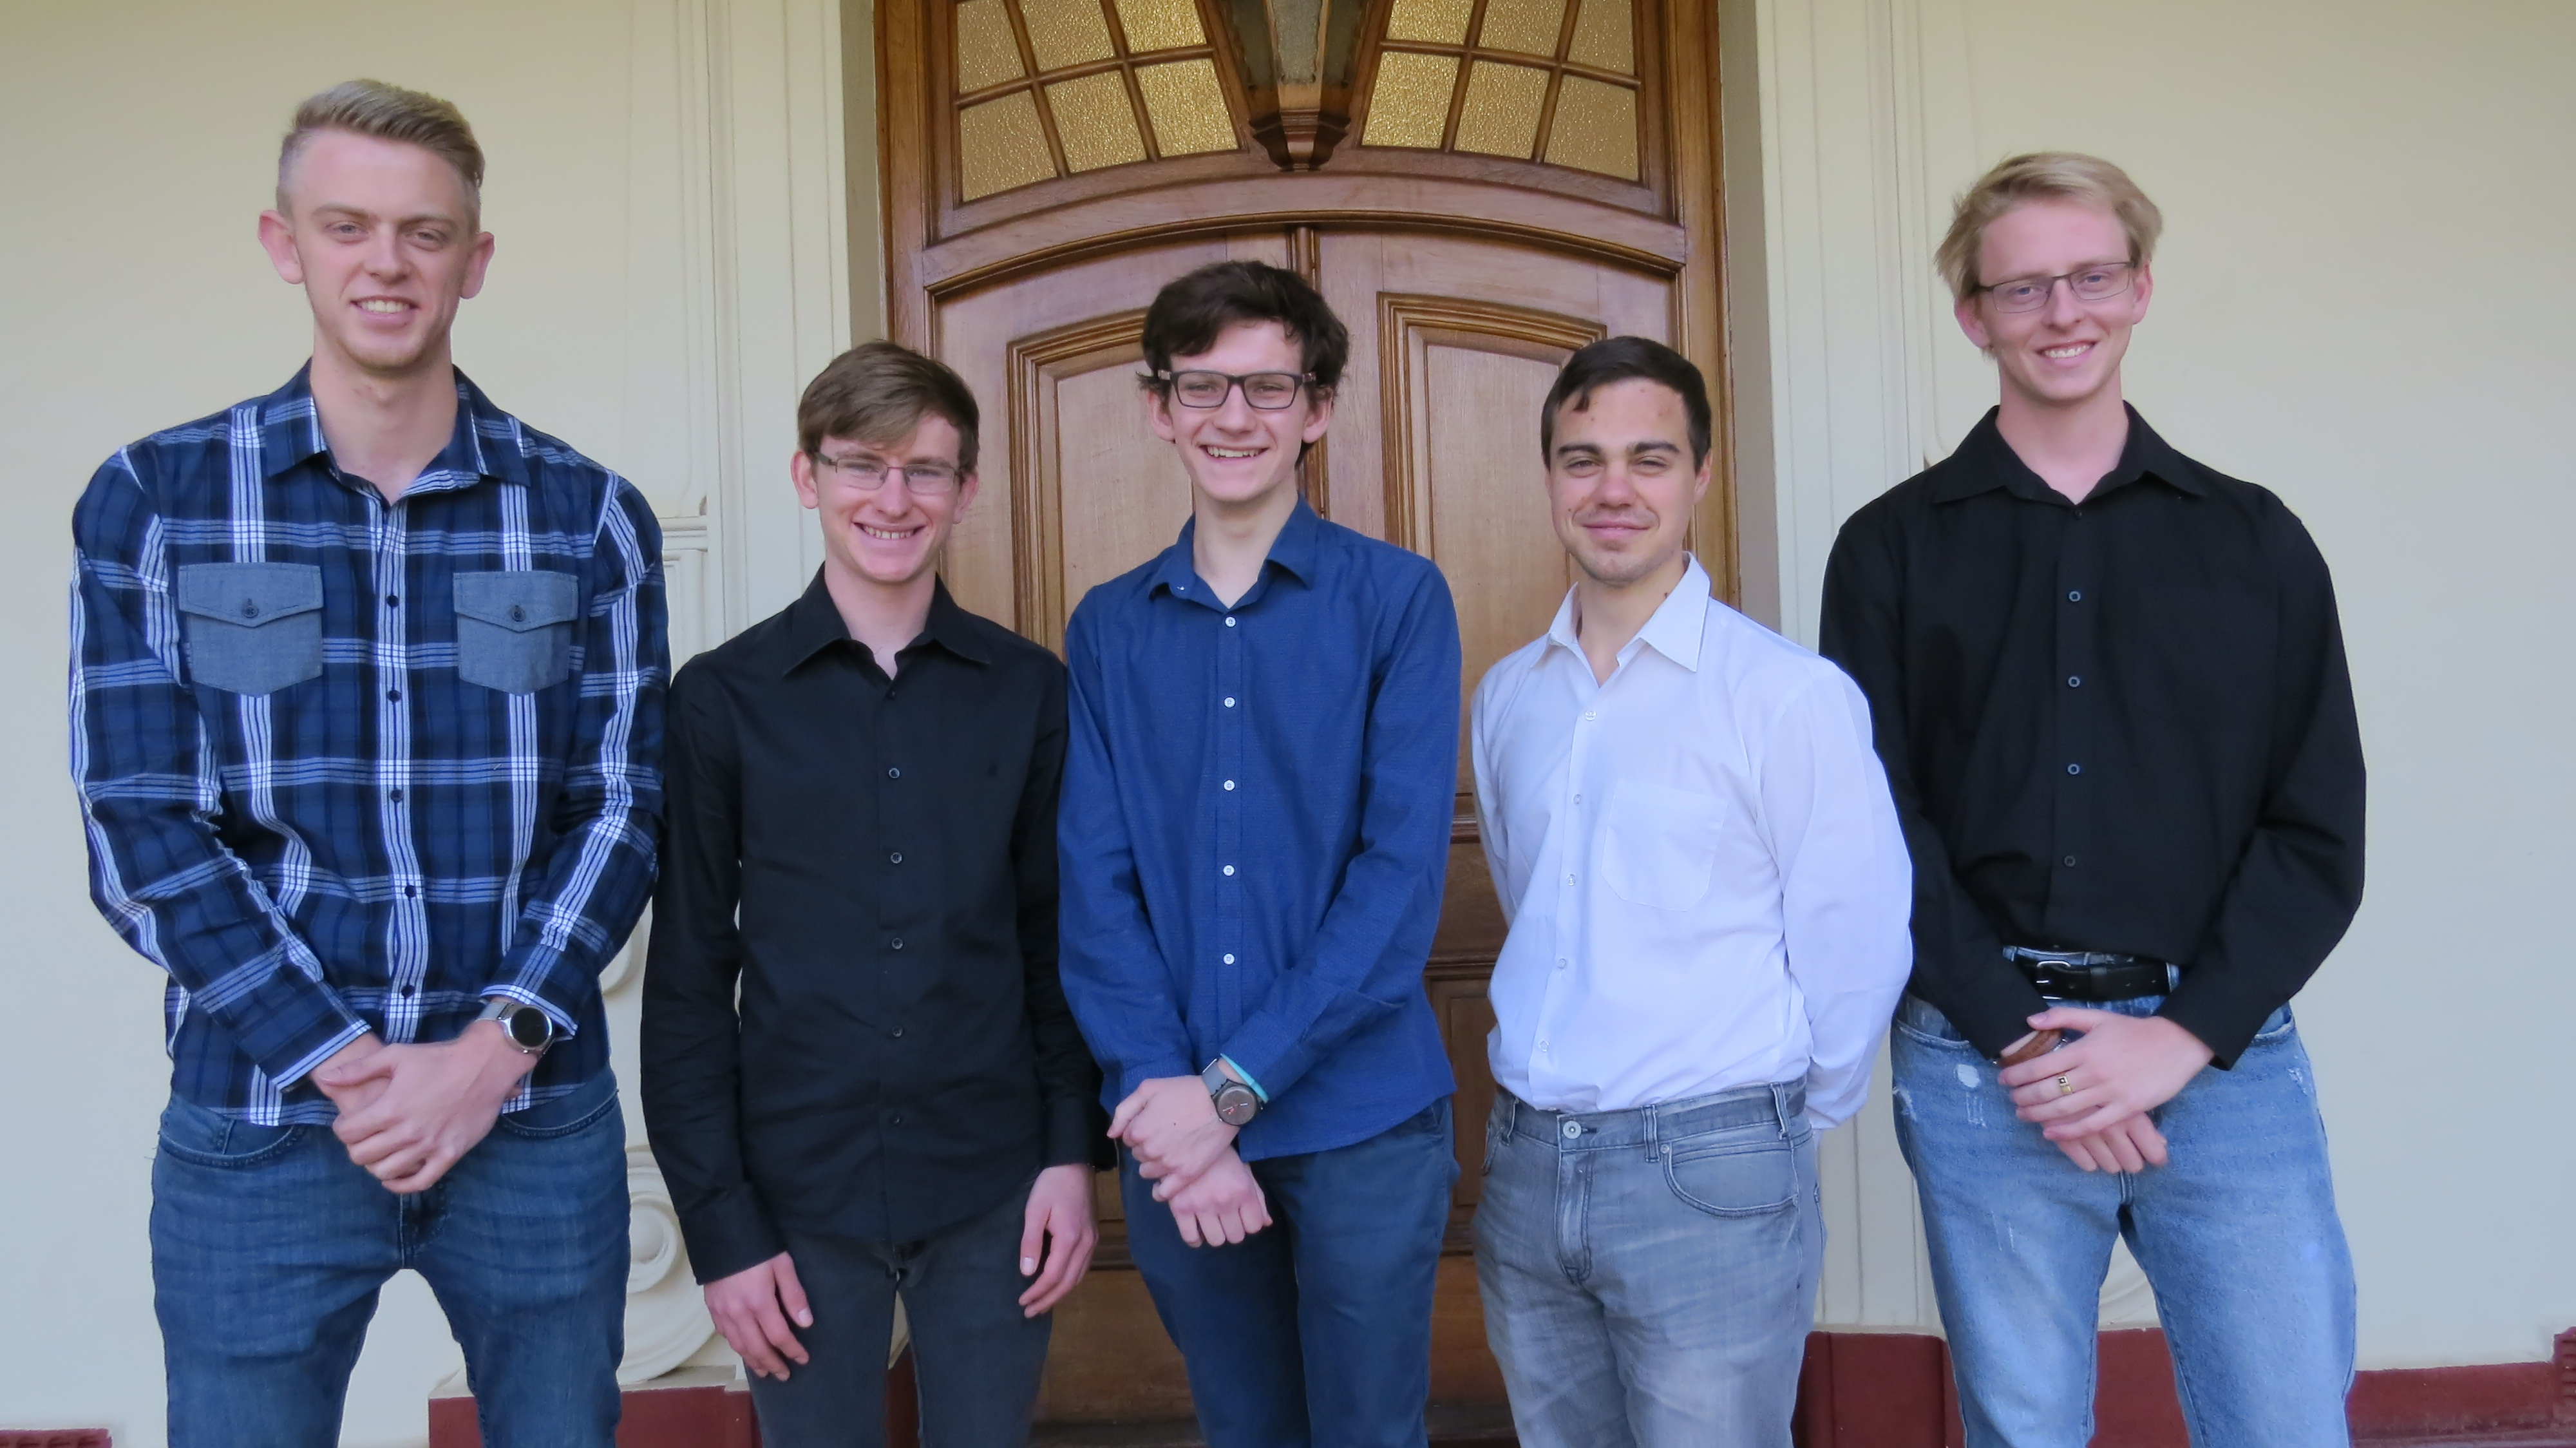
\includegraphics[width=\linewidth]{img/team_photo.jpg}}\\[2ex]
            {\large  Nicolai van Niekerk\\ \texttt{nicvaniek@gmail.com}}\\[2ex]
            {\large  Marno Hermann\\ \texttt{marno@barnton-consulting.co.za}}\\[2ex]
            {\large  Stephan Nell\\ \texttt{nellstephanj@gmail.com}}\\[2ex]
            {\large  Jan-Justin van Tonder\\ \texttt{J.vanTonder@tuks.co.za}}\\[2ex]
            {\large  Andreas Nel\\ \texttt{nel.andreas1@gmail.com}}\\[2ex]
        \end{center}
        
    \end{titlepage}
\makeatother

\cleardoublepage
\thispagestyle{empty}
\tableofcontents
\newpage

\section{Project Description}
    \lipsum[1]
    
    \lipsum[2]

\section{Execution}
    \subsection{Administrative Tasks}
        \subsubsection{Meetings}
            We firmly believe that active user involvement is imperative and will have frequent meetings with the client during development as well. We would like to work closely with the client to ensure that requirements misconceptions are corrected early on and that the client's feedback can be addressed properly and timely. The exact details and times of these meetings will be negotiated with the client. We do, however, think that it is imperative for at least the following meetings to happen:
            \begin{enumerate}
                \item As soon as the project is allocated and before the first demo (between 18 May 2017 and 25 May 2017)
                \item After the first demo (week of 29 May 2017 to 2 June 2017)
                \item In the week before or after the second demo (from 24 July 2017 to 4 August 2017)
                \item In the week before or after the third demo (from 28 August 2017 to 8 September 2017)
                \item In the week before the final evaluation phase starts (from 9 October 2017 to 13 October 2017)
            \end{enumerate}
    \subsection{Development}
        \subsubsection{Methodology}
        We plan on following the Agile Unified Methodology to implement this product. We will develop this product in iterations and strive to have a working prototype at all times. We feel that it is beneficial to adopt an iterative approach to our development rather than a sequential process like Waterfall. This will ensure that design issues and changes in requirements are identified early on, and will allow us to deliver a working system within our time constraints. We will have a brief planning phase in which we identify requirements, derive use cases and assign those use cases to iterations. Changes in requirements will be addressed during the requirements phase of each of the following iterations. We will have weekly team meetings and will have set meetings with the client after each iteration.
        \subsubsection{Technologies Used}
            \lipsum[1]
            
            \lipsum[2]
            
            \lipsum[3]
            
\newpage
\section{The Team}
    \subsection{Marno Hermann}
        \paragraph{Role} Developer
    
        \paragraph{Introduction}
            \begin{wrapfigure}{r}{0.5\textwidth}
              \begin{center}
                \vspace{-0.75cm}
                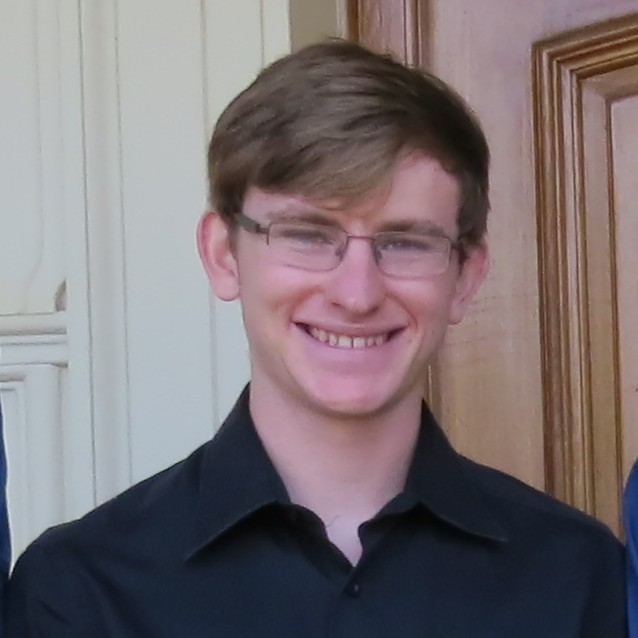
\includegraphics[width=0.5\textwidth]{img/marno.jpg}
              \end{center}
            \end{wrapfigure}
            I am a goal driven individual always trying to better myself and the people around me. Well balanced person that enjoys his morning runs. My passion for mathematics and solving puzzles ignited my interest in Artificial Intelligence. Specifically in optimisation since I have a knack for mathematics. Currently studying BscIT specialising in Applied Mathematics. I have developed several applications that is currently in use by different businesses in South Africa. I thus have experience in the development environment.   
        
        \paragraph{Skills}
            \begin{itemize}
                \item Programming languages: C++, Java, C\#, x86 Assembly, Delphi
                \item Extensive SQL knowledge
                \item Love to work in pressure situations
                \item Analytical Person
            \end{itemize}
            
        \paragraph{Achievements}
            \begin{itemize}
                \item I am a Microsoft Certified Technology Specialist (MCTS) completed 70-516 exam
                \item Golden key member
                \item 92\% for Matric 2014
                \item Second student in Department of Computer Science 2015
                \item GPA above 75\% for first and second years of study
                \item Finished Comrades 2016
                \item Through Barnton Consulting developed programs for SAB Miller, Premier Foods, Dartcom and RCL Foods.
            \end{itemize}
            
        \paragraph{Find me on the Web}
            \begin{itemize}
                \item \href{https://github.com/MarnoH}{Github} (https://github.com/MarnoH)
            \end{itemize}

\newpage        
    \subsection{Andreas Nel}
        \paragraph{Role} Code Reviewer
        \paragraph{Introduction}
        \begin{wrapfigure}{r}{0.5\textwidth}
            \begin{center}
            \vspace{-0.75cm}
            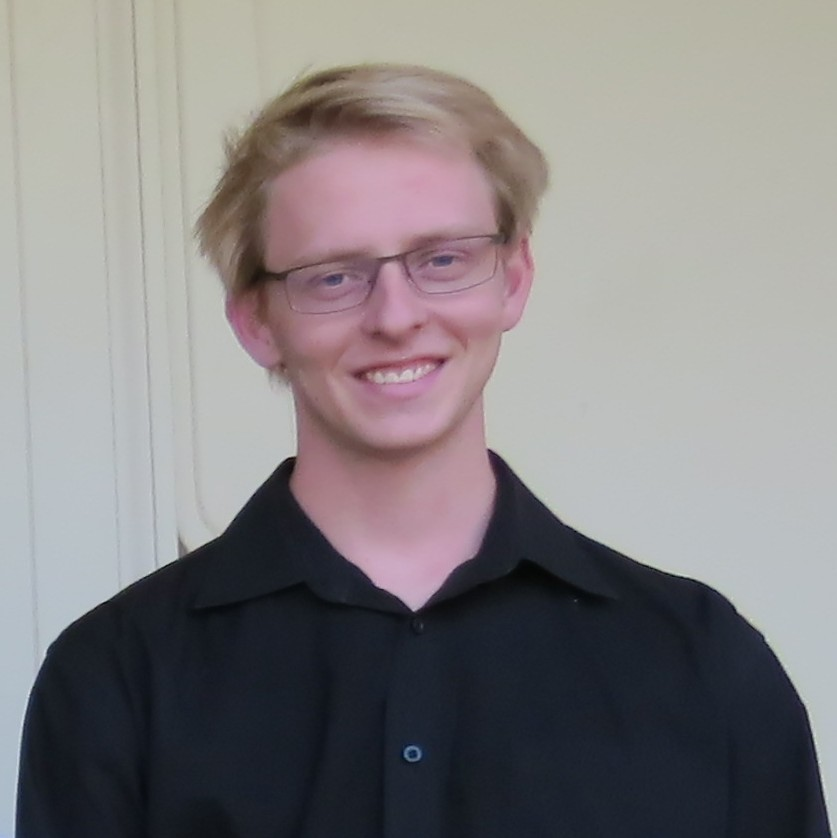
\includegraphics[width=0.5\textwidth]{img/andreas.jpg}
            \end{center}
        \end{wrapfigure}
        Ambitious, calculating, focused (with a tinge of dry humour). I spend a large amount of my time trying to improve my skill set and myself as a person, leading to me having held various positions in the past such as a sales person, waiter, research assistant and intern. I am extremely curious about the fields of Artificial Intelligence and Computer Security, and have quite recently also enjoyed working with computer networks.
        \paragraph{Skills}
            \begin{itemize}
                \item C++
                \item Java
                \item JavaScript (includes NodeJS, KnockoutJS)
                \item Bash Scripting
                \item Web Development
                \item SQL (includes MySQL, PostgreSQL)
                \item Object-Oriented Programming
            \end{itemize}
            
        \paragraph{Achievements}
            \begin{itemize}
                \item Golden Key member
                \item GPA above 75\% for both my first and second years of study
                \item One of the highest achievers in IT in Mpumalanga during the National Senior Certificate exams with an average of 96\%
                \item DUX learner Matric 2014
            \end{itemize}
            
        \paragraph{Find me on the Web}
            \begin{itemize}
                \item \href{https://github.com/AndreasNel}{GitHub} (https://github.com/AndreasNel)
                \item \href{https://www.linkedin.com/in/andreas-nel-340805130}{LinkedIn} (https://www.linkedin.com/in/andreas-nel-340805130)
            \end{itemize}
\newpage    
    \subsection{Stephan Nell}
        \paragraph{Role} Developer
        
        \paragraph{Introduction}
        \begin{wrapfigure}{r}{0.5\textwidth}
              \begin{center}
                \vspace{-0.75cm}
                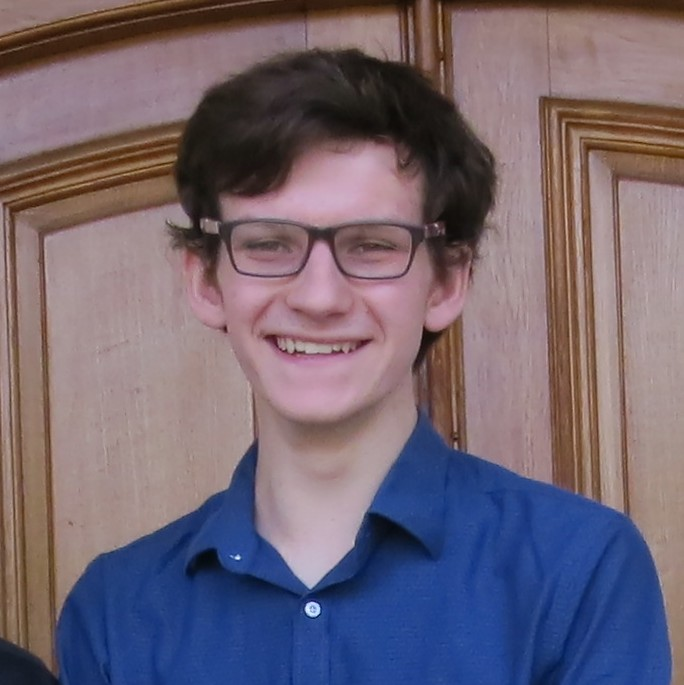
\includegraphics[width=0.5\textwidth]{img/stephan.jpg}
              \end{center}
            \end{wrapfigure}
            Calm and patient problem solver, who enjoys a good challenge. Always responsive to guidance and advice and seeking to make the most of my ability. I enjoy experimenting with new technologies and various networking problems. I am someone who collaborates well with others in a team and is always willing to go the extra mile to solve a problem and improve on current solutions. Currently, I enjoy my Networking and Artificial Intelligence courses, and I am determined to further my studies in Artificial Intelligence and Computer Security.
            
        \paragraph{Skills}
            \begin{itemize}
                \item C++
                \item Java
                \item Web Development
                \item SQL (includes MySQL, PostgreSQL)
                \item x86 Assembly
                \item Leadership
            \end{itemize}
            
        \paragraph{Achievements}
            \begin{itemize}
                \item Golden Key member
                \item GPA above 75\% for my second years of study.
            \end{itemize}
            
        \paragraph{Find me on the Web}
            \begin{itemize}
                \item \href{https://github.com/nellstephanj}{GitHub} (https://github.com/nellstephanj)
                \item \href{https://www.linkedin.com/in/stephan-nell-201710b8/}{LinkedIn} (https://www.linkedin.com/in/stephan-nell-201710b8/)
            \end{itemize}

\newpage    
    \subsection{Nicolai van Niekerk}
        \paragraph{Role} Team Lead 
        
        \paragraph{Introduction}
        \begin{wrapfigure}{r}{0.5\textwidth}
              \begin{center}
                \vspace{-0.75cm}
                
\includegraphics[width=0.5\textwidth]{img/nicolai.jpg}
              \end{center}
            \end{wrapfigure}
            Studying BSc IT specializing in software development, I have been exposed to the Systems Development Life Cycle since my first year at university. I am a quick learner and love to challenge myself to solve new problems and apply the knowledge that I have learnt. I love working in teams and have a particular passion for Software Engineering. I am very competitive and obsessed with developing myself in every aspect of my life.
            
        \paragraph{Skills}
            \begin{itemize}
                \item Good time and task management
                \item Good communication skills
                \item Quick learner
                \item Proficient in many programming languages including C++, Java, C\# and x86 Assembly
                \item Well versed in every aspect of the LAMP stack
                \item Experience with MEAN stack
                \item Database design and SQL
                \item Systems Analysis and Design
                \item UX Design
            \end{itemize}
            
        \paragraph{Achievements}
            \begin{itemize}
                \item DUX learner Matric 2014
                \item Top academic achiever TuksVillage residence 2015 with a GPA of 91.9\%
                \item Top student in Department of Computer Science 2015
                \item GPA above 85\% for first and second years of study
                \item Golden Key member
            \end{itemize}
            
        \paragraph{Find me on the Web}
            \begin{itemize}
                \item \href{https://github.com/Nicvaniek}{Github} (https://github.com/Nicvaniek)
                \item \href{https://www.linkedin.com/in/nicolai-van-niekerk-70970b109/}{Linkedin} (https://www.linkedin.com/in/nicolai-van-niekerk-70970b109/)
            \end{itemize}

\newpage
    \subsection{Jan-Justin van Tonder}
        \paragraph{Role} Developer
    
        \paragraph{Introduction}
        \begin{wrapfigure}{r}{0.5\textwidth}
              \begin{center}
                \vspace{-0.75cm}
                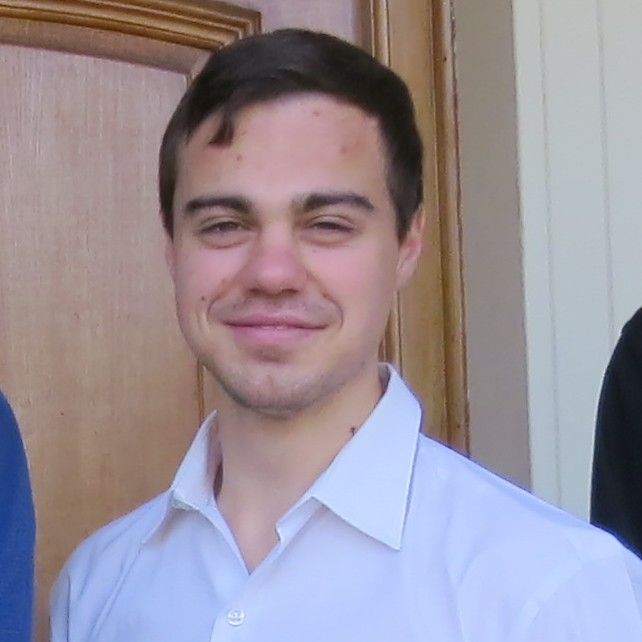
\includegraphics[width=0.5\textwidth]{img/justin.jpg}
              \end{center}
            \end{wrapfigure}
            Cool, calm, constant tinkerer and copious coffee drinker. I am constantly on the lookout for new challenges with a willingness to learn new, strange and wonderful things. I have a passion for computers and, in particular, Computer Networks as well as Artificial Intelligence. Being a BIT student, I have been exposed to the full spectrum of Information Technology, ranging from information science to computer science. I currently work as a Teaching Assistant for COS 216 (Netcentric Computer Systems) at the University of Pretoria.
            
        \paragraph{Skills}
            \begin{itemize}
                \item C++
                \item Java
                \item C\#
                \item SQL
                \item PHP
                \item Python
                \item MEAN stack
                \item Web Development
                \item Object-Orientated Modeling
                \item Systems Analysis and Design
            \end{itemize}
            
        \paragraph{Achievements}
            \begin{itemize}
                \item Top achiever for BIT on first year level 2015
                \item Top 5 academic achievers in Kollege residence 2015
                \item Golden Key member
                \item GPA above 75\% for first and second year
            \end{itemize}
            
        \paragraph{Find me on the Web}
            \begin{itemize}
                \item \href{https://github.com/jan-justin}{Github} (https://github.com/jan-justin)
                \item \href{https://www.linkedin.com/in/jan-justin-van-tonder-358bab142/}{Linkedin} (https://www.linkedin.com/in/jan-justin-van-tonder-358bab142/)
            \end{itemize}

\end{document}
